\documentclass[12pt]{article}

\usepackage[margin=1in]{geometry}
\usepackage{amsmath,amsthm,amssymb}
\usepackage{fancyhdr}
\usepackage[small,compact]{titlesec}
\usepackage{float}

\lhead{Erich Menge}
\chead{\classnameandsection}
\rhead{\homeworktitle}

\pagestyle{fancy}

\newcommand{\sethomeworknumber}[1]{
  \newcommand{\homeworktitle}{Homework #1}
}

\newcommand{\N}{\mathbb{N}}
\newcommand{\Z}{\mathbb{Z}}
\newcommand{\homeworkheader}[1]{
  \title{\vspace{2in}\homeworktitle}
  \author{Erich Menge (X.500: menge053, Student ID: 4624713) \\
  #1}
  \maketitle
  \newpage
}

\newenvironment{problem}[1]{
  \ignorespaces
  \section*{Problem #1}
}{
  \ignorespacesafterend
}

\newenvironment{solution}{
  \ignorespaces
  \subsection*{Solution}
}{
  \ignorespacesafterend
}

\newcommand{\classnameandsection}{CSCI 4011 Formal Languages And Automata Theory Section 3}

\usepackage{graphicx}
\usepackage{subfigure}

\sethomeworknumber{1}

\begin{document}

\begin{problem}{1.6}

  Scrooge McNugget wants to store information (names, addresses, descriptions of embarrassing moments, etc.) about the
  many ducks on his payroll. Not surprisingly, the volume of data compels him to buy a database system. To save money,
  he wants to buy one with the fewest possible features, and he plans to run it as a stand-alone application on his PC
  clone. Of course, Scrooge does not plan to share his list with anyone. Indicate which of the following DBMS features
  Scrooge should pay for; in each case, also indicate why Scrooge should (or should not) pay for that feature in the
  system he buys.

  \begin{enumerate}
    \item A security facility.
    \item Concurrency control.
    \item Crash recovery.
    \item A view mechanism.
    \item A query language.
  \end{enumerate}

  \begin{solution}
    \begin{enumerate}
      \item Yes. He's putting it on his PC ``clone''. Because it is standalone and no one else needs to access it
      it should not accept network connections and should be located in a physically secure location. Physical access
      is total access.

      \item No. Since it is single-user there is no need for concurrency.

      \item Yes. Despite his frugality he is storing very valuable information (embarrassing moments) which he probably
      can't afford to lose. It would be good to make sure that in the event of a power outage his data isn't corrupted.

      \item Yes. While not strictly necessary, it may make Scrooge's life easier to create views. It doesn't specify
      if he will be using a program or accessing his database directly. If he is accessing it directly it may make sense
      for him to have views so that his work environment isn't as cluttered with less frequently used columns for instance.

      \item Yes. He will need to use the query language to interact with his database.
    \end{enumerate}
  \end{solution}
\end{problem}

\begin{problem}{2.2}

  A university database contains information about professors (identified by social security number, or SSN) and
  courses (identified by courseid). Professors teach courses; each of the following situations concerns the Teaches
  relationship set. For each situation, draw an ER diagram that describes it (assuming no further constraints hold).

  \begin{enumerate}
    \item Professors can teach the same course in several semesters, and each offering must be recorded.
    \item Professors can teach the same course in several semesters, and only the most recent such offering needs to be
      recorded. (Assume this condition applies in all subsequent questions.)
    \item Every professor must teach some course.
    \item Every professor teaches exactly one course (no more, no less).
    \item Every professor teaches exactly one course (no more, no less), and every course must be taught by some professor.
    \item Now suppose that certain courses can be taught by a team of professors jointly, but it is possible that no one
      professor in a team can teach the course. Model this situation, introducing additional entity sets and relationship
      sets if necessary.
  \end{enumerate}

  \begin{solution}
    \begin{figure}[H]
      \centering
      \subfigure[ER Diagram for 2.2-1]{
        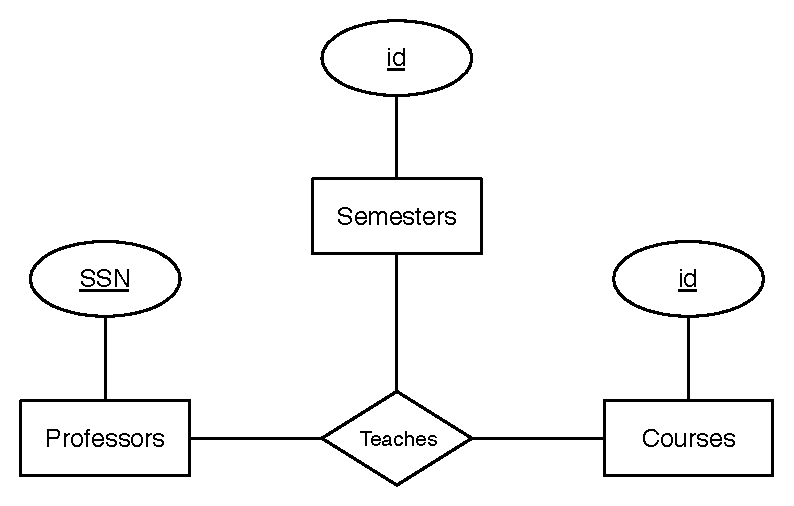
\includegraphics[scale=.5]{2_2_1.eps}
      } \qquad
      \subfigure[ER Diagram for 2.2-2]{
        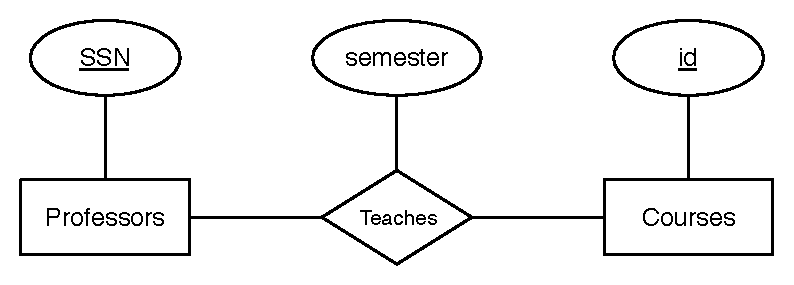
\includegraphics[scale=.5]{2_2_2.eps}
      } \qquad
      \subfigure[ER Diagram for 2.2-3]{
        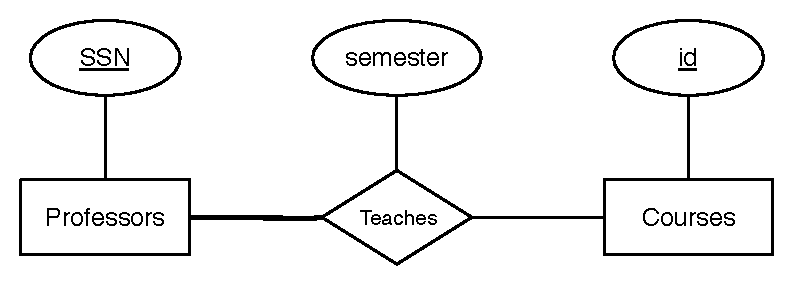
\includegraphics[scale=.5]{2_2_3.eps}
      } \qquad
      \subfigure[ER Diagram for 2.2-4]{
        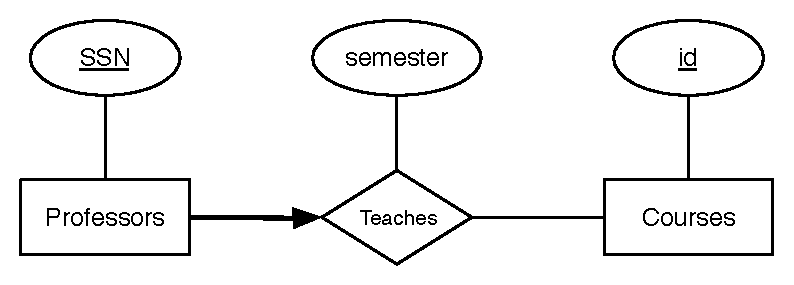
\includegraphics[scale=.5]{2_2_4.eps}
      } \qquad
      \subfigure[ER Diagram for 2.2-5]{
        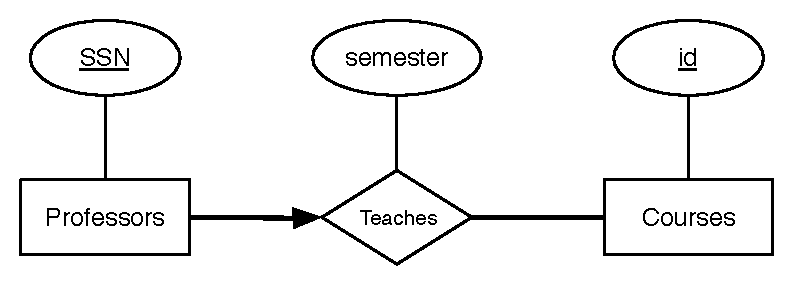
\includegraphics[scale=.5]{2_2_5.eps}
      } \qquad
      \subfigure[ER Diagram for 2.2-6]{
        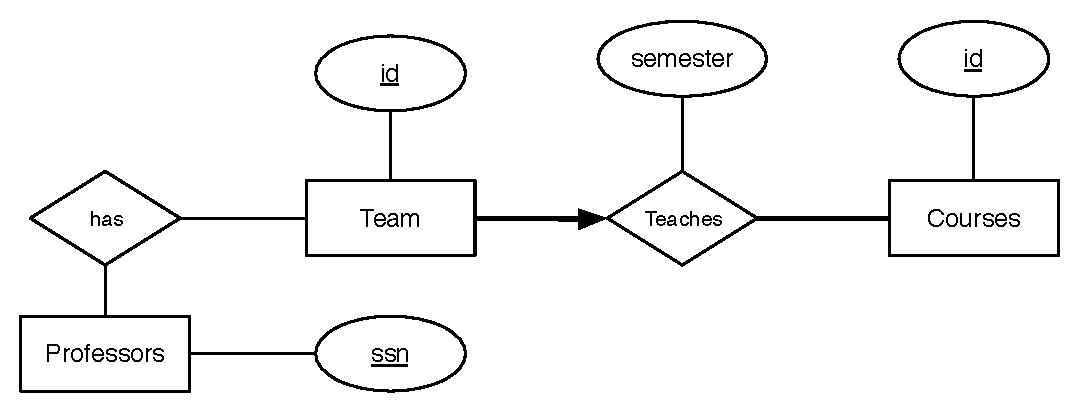
\includegraphics[scale=.5]{2_2_6.eps}
      } \qquad
    \end{figure}
  \end{solution}
\end{problem}
\begin{problem}{2.4}
  \begin{solution}
  \end{solution}
\end{problem}
\begin{problem}{2.6 (1)}
  \begin{solution}
  \end{solution}
\end{problem}
\begin{problem}{2.8}
  \begin{solution}
  \end{solution}
\end{problem}


\end{document}
